\documentclass{article}
\usepackage{lmodern}
\usepackage{amsmath}
\usepackage{amssymb}
\usepackage[T1]{fontenc}
\usepackage{listings}
\usepackage{fancyhdr}
\usepackage{hyperref}
\usepackage{pdfpages}

\pagestyle{fancy}
\lhead{Anirudhan J Rajagopalan - ajr619 - N18824115} % chktex 8

\begin{document}

\title{Foundations of Machine Learning --- Homework Assignment 1}
\date{November 08, 2015}
\author{Anirudhan J Rajagopalan\\ N18824115\\ ajr619}

\maketitle

\newpage

\section*{C. Support Vector Machines}
\subsection*{1}
Installed the software from\cite{libsvm}.  The installed version of software is also checked into github at\cite{githuburl}. 
\subsection*{2}

\noindent See the following command:
\begin{lstlisting}[language=bash]
  $ ./svm-scale -s splice_noise_train.txt.range \  
  > splice_noise_train.txt > splice_noise_train.txt.scale
  $ ./svm-scale -r splice_noise_train.txt.range \
  > splice_noise_test.txt > splice_noise_test.txt.scale
\end{lstlisting}

\subsection*{3}
Run training and test script\cite{cvscript} by editing the KERNEL\_DEGREE parameter for each value of d = 1, 3, 5.
\begin{lstlisting}
  $ python cross_validation.py > deg1.out # KERNEL_DEGREE = 1
  $ python cross_validation.py > deg3.out # KERNEL_DEGREE = 3
  $ python cross_validation.py > deg5.out # KERNEL_DEGREE = 5
\end{lstlisting}

Filter the parameter and accuracy information from the run logs (deg1.out, deg3.out and deg5.out) by the command below.
\begin{lstlisting}
  $ cat deg1.out | grep OUR | cut -d' ' \
  > -f2,3,4,5,6 > deg1.out.filtered
  $ cat deg3.out | grep OUR | cut -d' ' \
  > -f2,3,4,5,6 > deg3.out.filtered
  $ cat deg5.out | grep OUR | cut -d' ' \
  > -f2,3,4,5,6 > deg5.out.filtered
\end{lstlisting}

Use plotter.py\cite{plotterpy} to create plots from the output values for KERNEL\_DEGREE values 1, 3, 5.  The output will be saved as deg1.pdf, deg3.pdf and deg5.pdf.  All the three plots are embedded below one after the other.  The dotted red line corresponds to -1 standard deviation.  The dotted green line corresponds to +1 standard deviation and the black continuous line corresponds to the Mean.
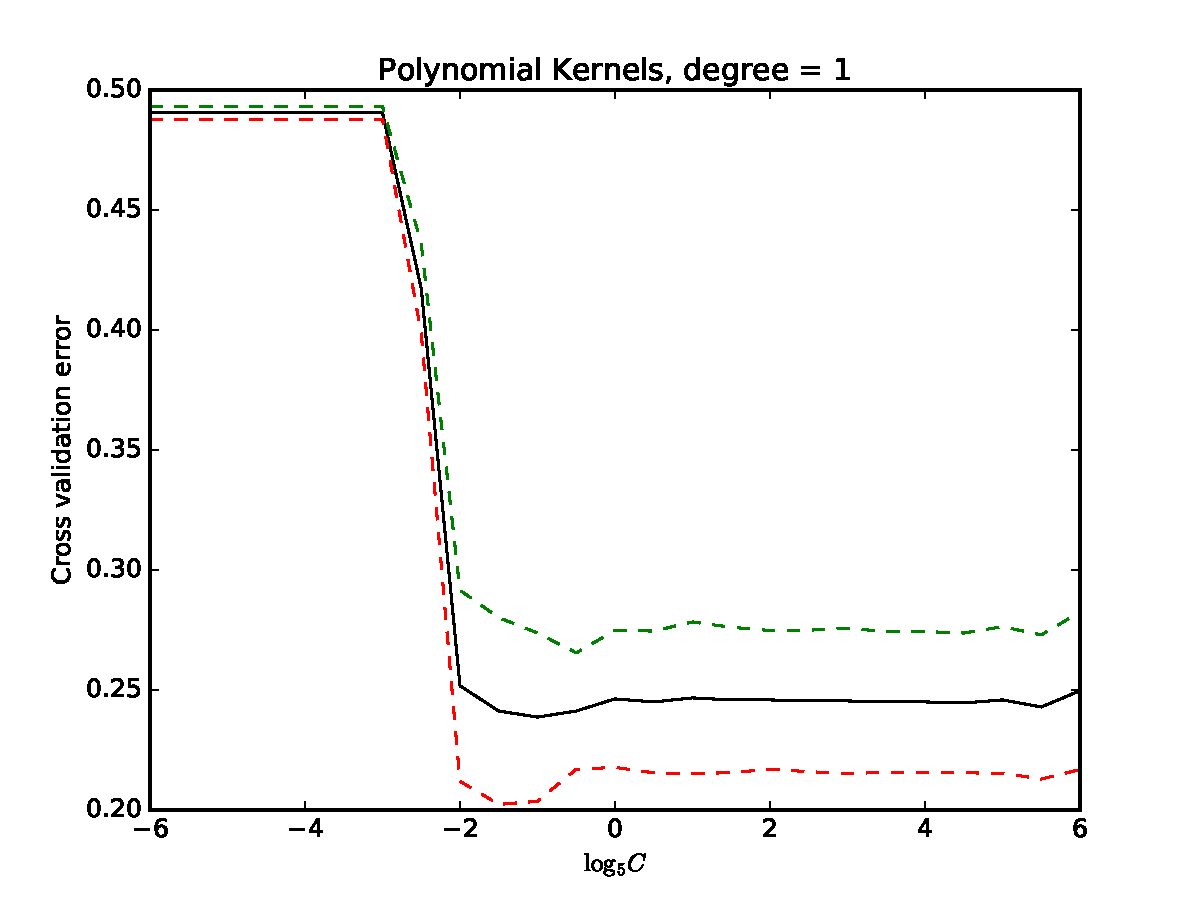
\includepdf[pages={1},lastpage={1}]{libsvm-3.20/tools/deg1.pdf}
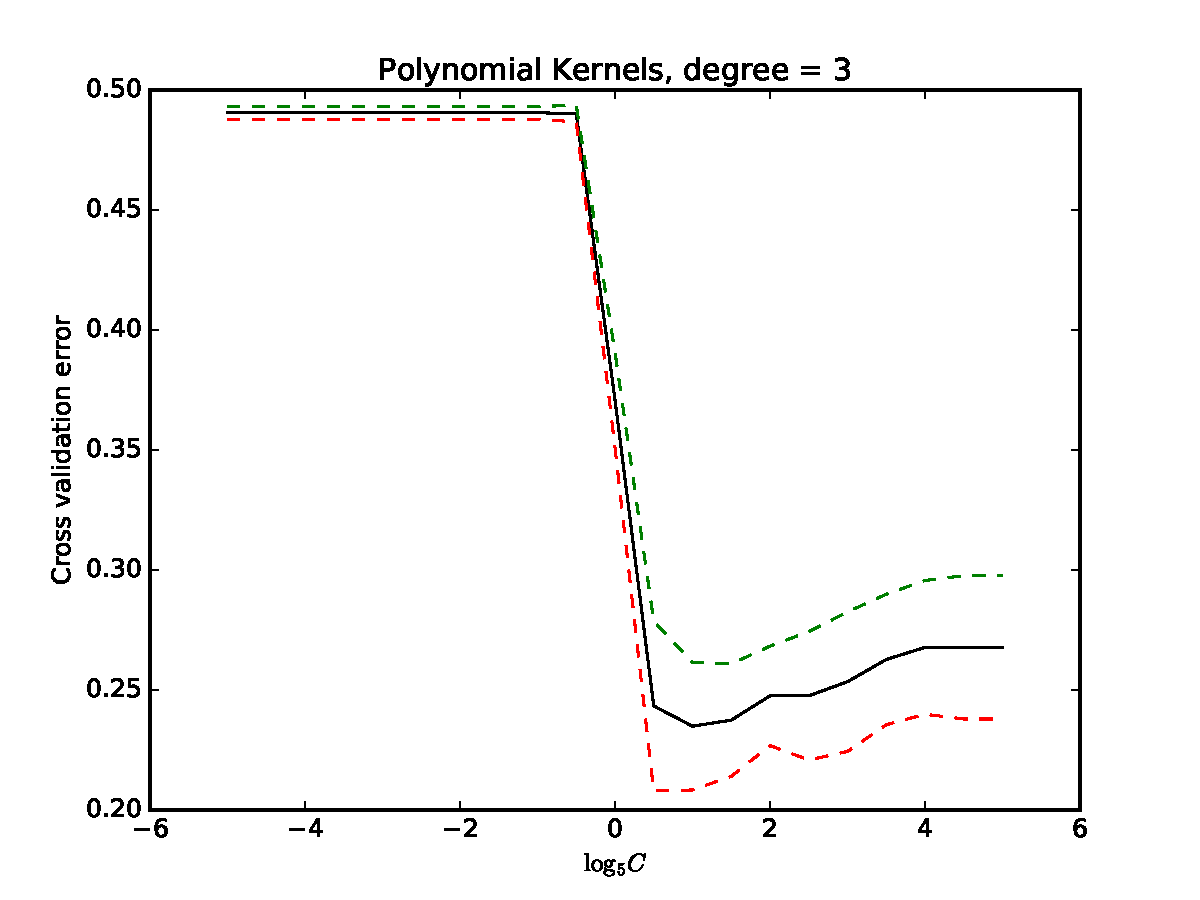
\includepdf[pages={1},lastpage={1}]{libsvm-3.20/tools/deg3.pdf}
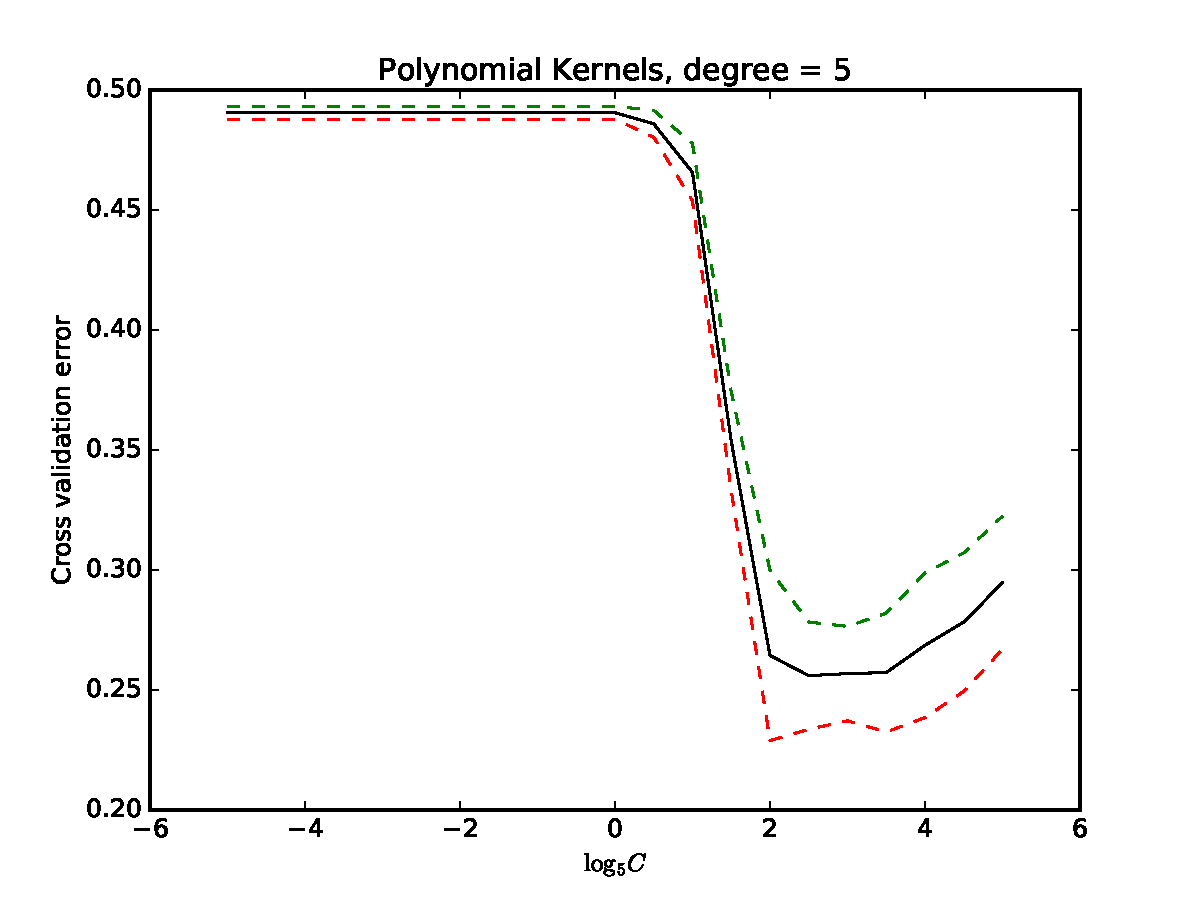
\includepdf[pages={1},lastpage={1}]{libsvm-3.20/tools/deg5.pdf}

Best values of c for polynomial kernels 1, 3, 5 are:
\begin{align*}
  d = 1 && c* = 5^{-1.0} = 0.2 && \mathrm{cv-err} = 23.87\% \pm 3.5\% \\
  d = 3 && c = 5^{1.0} = 5 && \mathrm{cv-err} = 23.49\% \pm 2.65\%\\
  d = 5 && c = 5^{2.5} = 55.9017 && \mathrm{cv-err} = 25.59\% \pm 2.23\% \\
\end{align*}

The best C measured in the cross-validation set is \( C^{*} = 5^{1.0} \) with degree \( d^{*} = 3 \) which gives an average error of \( 23.49\% \pm 2.65\% \)

\subsection*{4}
The average number of SV and BSV are taken across the cross validation sets.  NumMarginal represents the average number of marginal support vectors.

Similarly nSV and nBSV represent the number of support vectors and bounded support vectors in test set.  Marginal represents the number of support vectors in test set.

After manually populating d, cross-train accuracy, test accuracy, nSV, nBSV, rho, totalSV, totalBSV into a file\cite{ques4file}, we run a script\cite{ques4py} to generate the plots as a pdf file.

\begin{tabular}{*{7}{c}}
  D & Avg Sv & Avg BSV & numMarginal & nSv & nBSV & marginal \\
  1 & 1241.3 & 1175.4 & 65.9 & 1377 & 1309 & 68 \\
  3 & 1990.5 & 1042.7 & 947.8 & 2183 & 1138 & 1045 \\
  5 & 2132.4 & 1937.4 & 195.0 & 2368 & 2150 & 218 \\
\end{tabular}

Soft margin is given by the rho value.  Svm-train outputs negative margin values (rho). We use rho values to plot the soft margins in our plots.
The plots generated are as shown below.

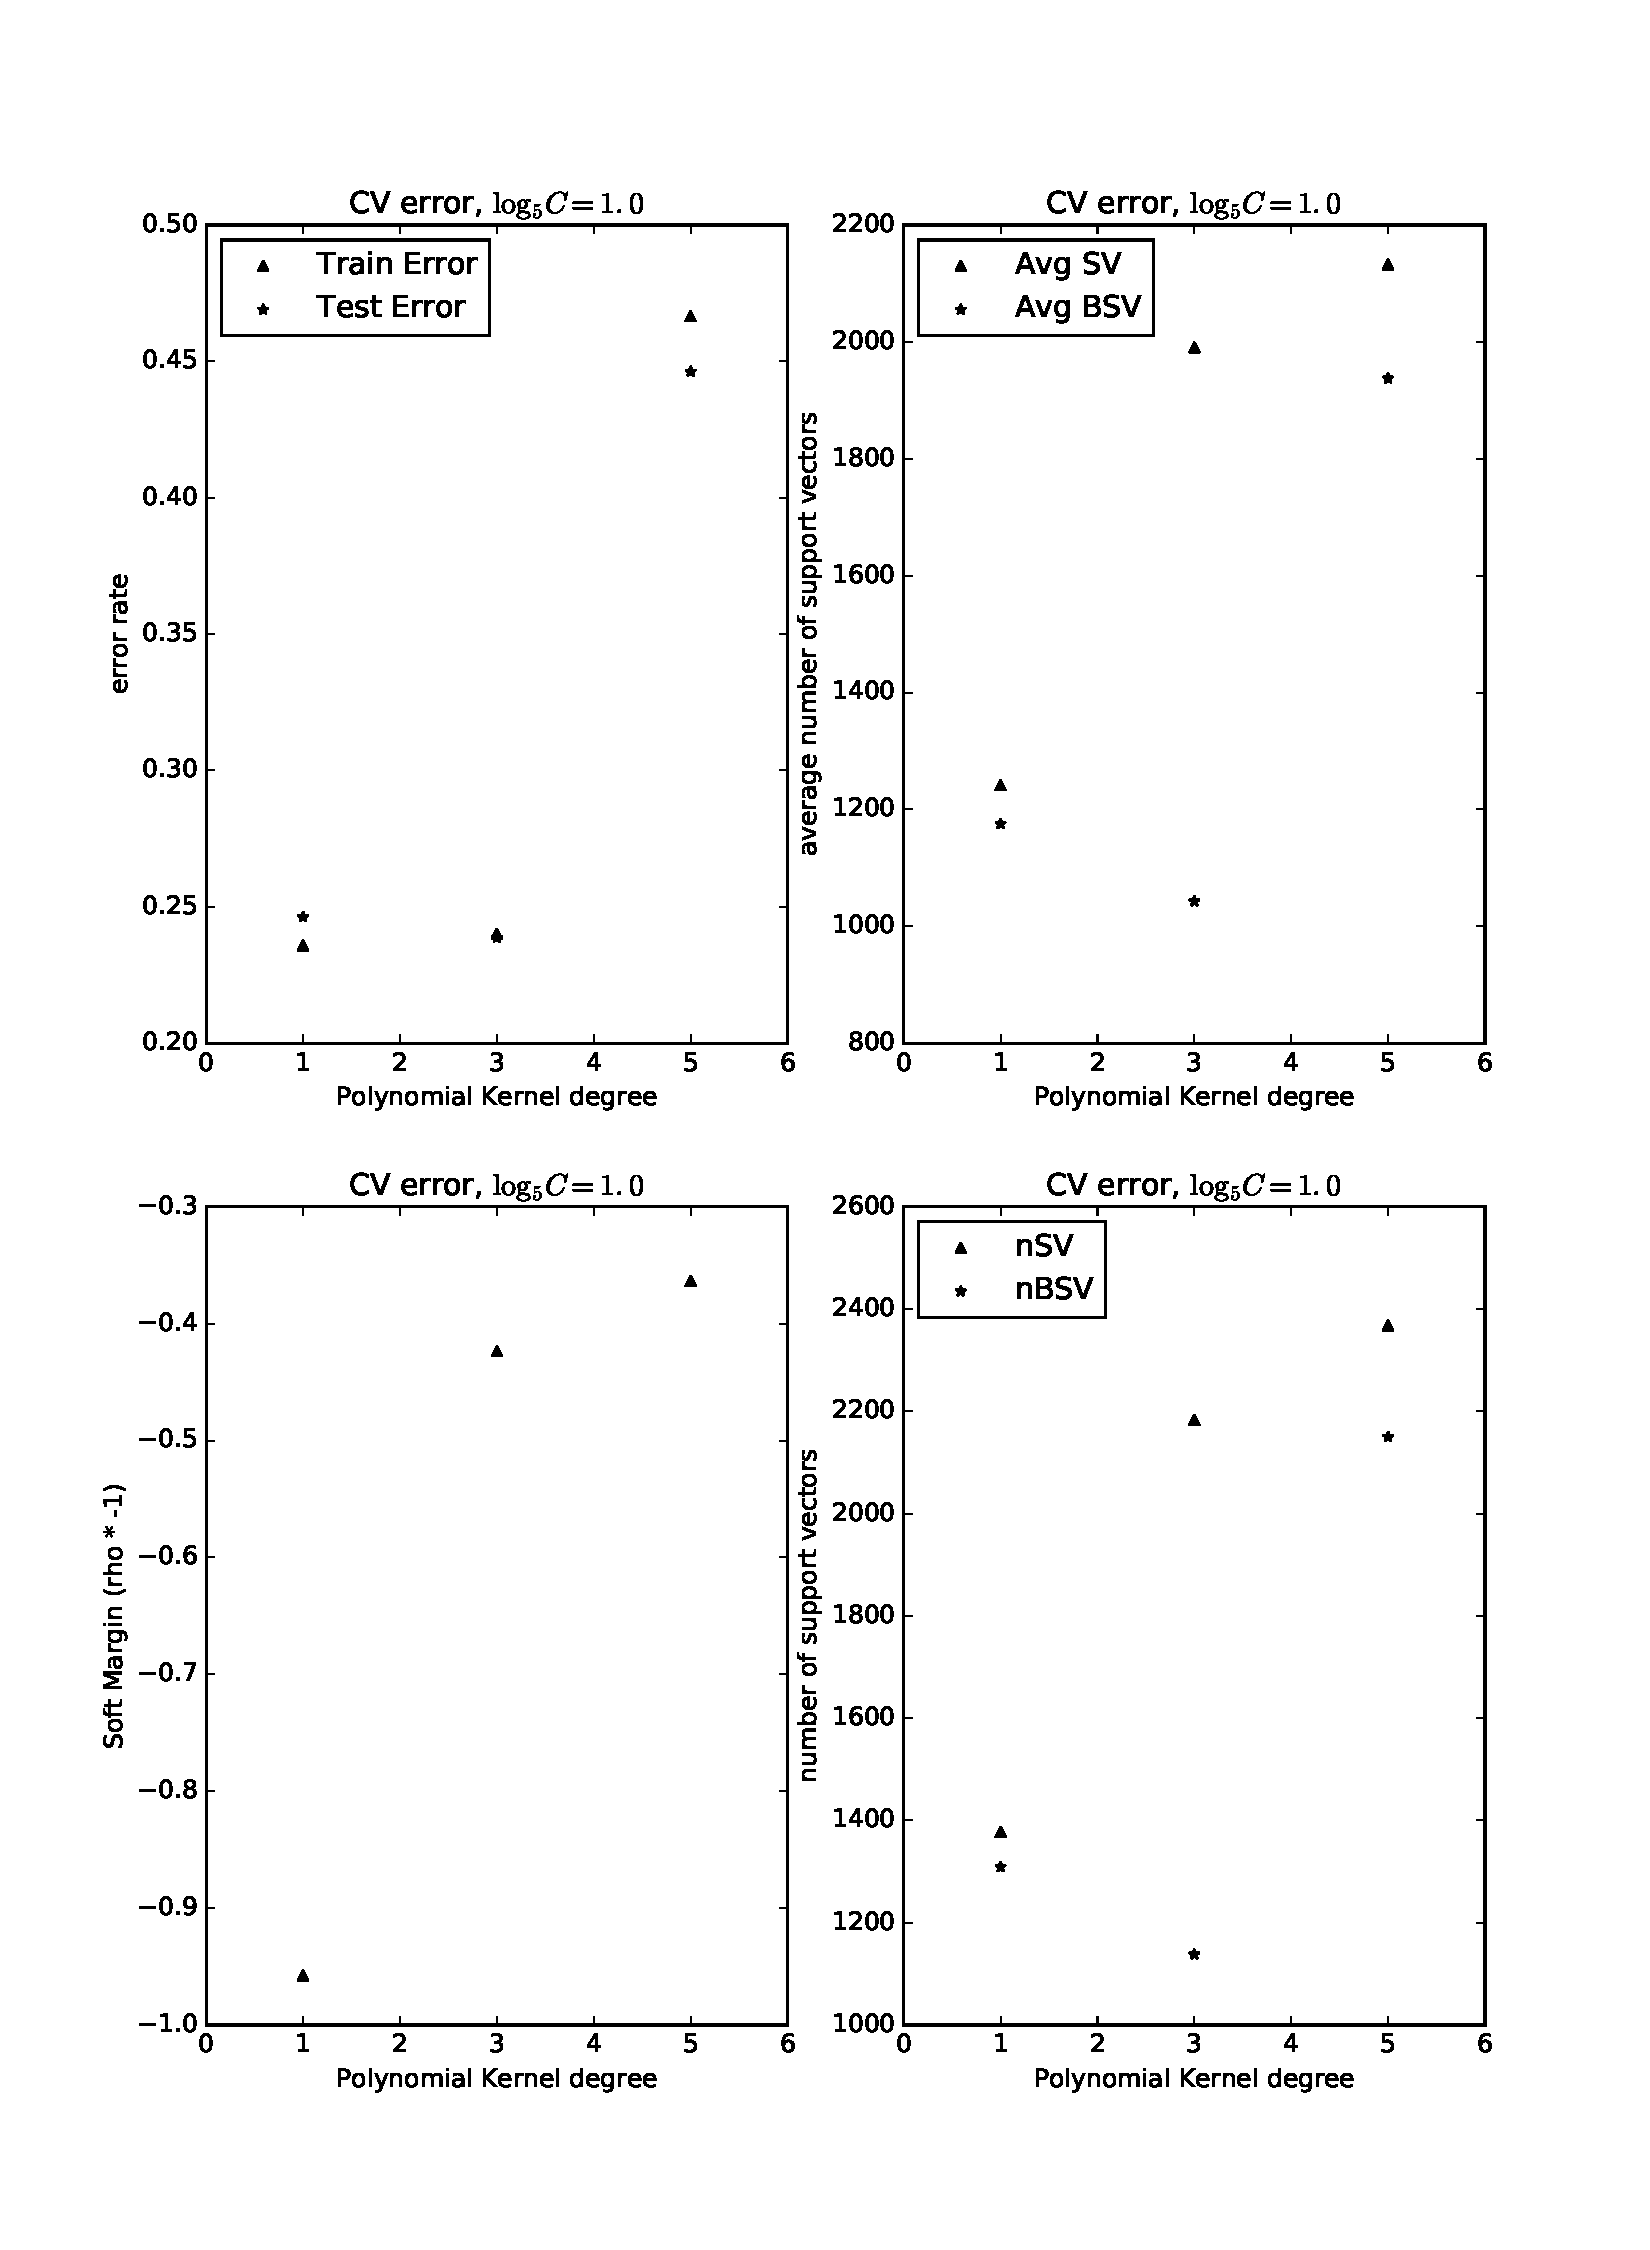
\includepdf[pages={1},lastpage={1}]{libsvm-3.20/tools/ques4_1.pdf}
\subsection*{5}
We can modify grid.py to use `C' in powers of 5 (change 2**c to 5**c in lines 142, 262, 348, 453 and 454).
Running grid.py with -log5c -4,4,1 and -log2g -4,4,1 -v 10 -t 2, -s 0 gives us the best value of c and g.

We get the best cross validation accuracy of 79.7474 for c = 1.0 and g = 0.03125.  Note that \( \sigma = \sqrt{\frac{1}{2g}} \)

We train the svm with the obtained c and v values
\begin{lstlisting}
  $ ./svm-train -t 2 -s 0 -c 1.0 -g 0.03125 \
  > ./splice_hw/splice_noise_train.txt.scale ./rbf.model
  $ ./svm-predict \./splice_hw/splice_noise_test.txt.scale \
  > rbf.model rbf.output
\end{lstlisting}
gives us Accuracy = 80.125\% (641/800) (classification)

The best accuracy we got with polynomial kernel SVM is 76.125 for \( C^{*} = 5^{1.0} \) with degree \( d^{*} = 3 \).

The value of soft margin (rho) for the rbf kernel SVM is -0.586184.

\subsection*{6}

\section*{D. Kernels}
\subsection*{1}
\begin{description}
  \item{Given:} Kernel, K is defined by \(K(x,y) = \sum_{i=1}^{N} \cos^{n} (x_{i}^{2} - y_{i}^{2} )\) for all \((X, Y) \in \mathbb{R}^{N} \times \mathbb{R}^{N} \) 
  \item{Solution:}  We know that
    \begin{equation}
      \cos (x_{i}^{2} - y_{i}^{2}) = \sin (x_{i}^{2}).\sin (y_{i}^{2}) + \cos (x_{i}^{2}).\cos (y_{i}^{2})
    \end{equation}
    This can be written as a dot product of two vectors 
    \begin{align}
    \phi(x_{i}) = \begin{bmatrix} \cos (x_{i}^{2}) \\ \sin (x_{i}^{2}) \end{bmatrix} && \mathrm{and} &&
    \phi(y_{i}) = \begin{bmatrix} \cos (y_{i}^{2}) \\ \sin (y_{i}^{2}) \end{bmatrix}
    \end{align}

    K can be written as summation of N kernels that are a product of n \( K^{'} \) kernels.  \( K' = \cos (x_{i}^{2} - y_{i}^{2} ) \).  Hence to prove that K is PDS, it is enough to show that \( K^{'} \) is PDS. 

    To show \( K^{'}\) is PDS, we show that \( c^{T}K'c \)  > 0 for any column vector \( C = (C_{1}, C_{2}, ...  ,C_{m})^{T} \in \mathbb{R}^{m} ) \)

    \begin{align}
    C^{T}K^{'}C  =& \sum_{i,j = 1}^{m} c_{i}c_{j} \begin{bmatrix} \cos (x_{i}^{2}) \\ \sin (x_{i}^{2}) \end{bmatrix} \begin{bmatrix} \cos (y_{i}^{2}) \\ \sin (y_{i}^{2}) \end{bmatrix} \\
      =& \sum_{i=1}^{n}c_{i} \begin{bmatrix} \cos (x_{i}^{2}) \\ \sin (x_{i}^{2}) \end{bmatrix} \times \sum_{j=1}^{n}c_{j} \begin{bmatrix} \cos (y_{j}^{2}) \\ \sin (y_{j}^{2}) \end{bmatrix}\\
    =& \begin{bmatrix} \sum_{i=1}^{n} c_{i} \begin{bmatrix} \cos (x_{i}^{2}) \\ \sin (x_{i}^{2})  \end{bmatrix} \end{bmatrix}^{2} \\
    \ge& 0
    \end{align}

    Which proves \( K^{'} \) is PDS. 


    Hence \( K(x,y) = \sum_{i=1}^{N} \cos^{n} (x_{i}^{2} - y_{i}^{2} ) \) is PDS.
\end{description}

\subsection*{1}
\begin{description}
  \item{Given:} \( K(x,y) = e^{-\frac{ \left\lVert x - y \right\rVert }{\sigma}} \) \\
    and \( \left\lVert x - y \right\rVert  = \frac{1}{2\Gamma{\frac{1}{2}}} \int_{0}^{\infty} \frac{1 - e^{-t(\left\lVert x - y \right\rVert^{2})} }{ t^{3/2}} dt \) valid for all x,y
  \item{To prove:} K is PDS
  \item{Proof:}
    A normalized kernel $K^{'}$ for any kernel K is given by
    \begin{equation*}
      K^{'} = \frac{K(x,y)}{\sqrt{K(x,x) K(y,y)}}
    \end{equation*}

    For a PDS kernel given by K1 = $e^{2txy} \forall t \ge 0$ we have the normalized kernel $K_{1}$as 
    \begin{align}
      =& \frac{e^{2txy}}{\sqrt{e^{2tx.x}e^{2ty.y}}} \\
      =& \frac{e^{2txy}}{e^{t(x.x + y.y)}} \\
      =& e^{-t(\left\lVert x - y \right\rVert^{2})}
    \end{align}

    Since K1 is PDS, its normalized kernel $K_{1} $ is also a PDS kernel.

    => $-e^{-t(\left\lVert x - y \right\rVert^{2})}$ is NDS and also 1 $-e^{-t(\left\lVert x - y \right\rVert^{2})}$ is also NDS.  Since $ t \ge 0$, we can say that $ K_{nds} = \frac{1 - e^{-t(\left\lVert x - y \right\rVert^{2})}}{t^{3/2}}$ is also a NDS kernel.

    Now, for the kernel $K_{2} = \frac{1}{2\Gamma{\frac{1}{2}}} \int_{0}^{\infty} \frac{1 - e^{-t(\left\lVert x - y \right\rVert^{2})} }{ t^{3/2}} dt$
    for any column vector \( C = (C_{1}, C_{2}, ...  ,C_{m})^{T} \in \mathbb{R}^{m} ) \)
    \begin{align*}
      C^{T}K_{2}C =& \sum_{i,j=1}^{n} c_{i}c_{j} K_{2}(x_{i}x_{j}) \\
      =& \sum_{i,j=1}^{n} c_{i}c_{j} \bigl[ \frac{1}{2\Gamma{\frac{1}{2}}} \int_{0}^{\infty} \frac{1 - e^{-t(\left\lVert x - y \right\rVert^{2})} }{ t^{3/2}} dt \bigr] \\
      =& \frac{1}{2\Gamma{\frac{1}{2}}} \bigl[ \int_{0}^{\infty} \sum_{i,j=1}^{n} c_{i}c_{j} \frac{1 - e^{-t(\left\lVert x - y \right\rVert^{2})} }{ t^{3/2}} dt \bigr] 
    \end{align*}
    Since we know that $K_{nds} \le 0$; 
    \begin{align*}
      C^{T}K_{2}C \le& 0 \\
    \end{align*}
    => $K_{2}$ is also NDS.

    This proves that \( \left\lVert x - y \right\rVert \) is an NDS kernel.  Since \( \left\lVert x - y \right\rVert \) is NDS, from lecture5 which states that K is NDS iff exp(-tK) is PDS for all t > 0: 

    => $e^{-t\left\lVert x - y \right\rVert} $  is a PDS kernel where $t = \frac{1}{\sigma} $
\end{description}

\begin{thebibliography}{1}
  \bibitem{libsvm} \url{http://www.csie.ntu.edu.tw/~cjlin/libsvm/}
  \bibitem{githuburl} \url{http://git.io/v80yn}
  \bibitem{cvscript} \url{http://git.io/v80yY}
  \bibitem{plotterpy} \url{http://git.io/v80yk}
  \bibitem{ques4file} \url{http://git.io/v8Edr}
  \bibitem{ques4py} \url{http://git.io/v8EdH}
  \bibitem{kerneladder} \url{http://git.io/v8KT1}
\end{thebibliography}

\end{document}
